
\documentclass[a4paper,fleqn]{cas-dc}
\usepackage[section]{placeins}
\usepackage[authoryear,longnamesfirst]{natbib}

%%%Author definitions
\def\tsc#1{\csdef{#1}{\textsc{\lowercase{#1}}\xspace}}
\tsc{WGM}
\tsc{QE}
\tsc{EP}
\tsc{PMS}
\tsc{BEC}
\tsc{DE}
%%%

% Uncomment and use as if needed
%\newtheorem{theorem}{Theorem}
%\newtheorem{lemma}[theorem]{Lemma}
%\newdefinition{rmk}{Remark}
%\newproof{pf}{Proof}
%\newproof{pot}{Proof of Theorem \ref{thm}}

\begin{document}
\let\WriteBookmarks\relax
\def\floatpagepagefraction{1}
\def\textpagefraction{.001}

\shorttitle{Detekcja Anomalii}

% Main title of the paper
\title [mode = title]{Detekcja Anomalii w Członkostwach Miast w Sieciach Transnarodowych za Pomocą Sztucznej Inteligencji}                      


\author[1]{Rzyszka Kamil}[role=xxx]

% Address/affiliation
\affiliation[1]{organization={Zieloni VaBanque},
    addressline={Prószkowska 29}, 
    city={Opole},
    postcode={45-962}, 
    country={Poland}}

% Second author
\author[1]{Seniush Yevhenii}[role=xxx]

% Third author
\author[1]{Skowron Dawid}[role=xxx]

% Fourth author
\author[1]{Żuliński Marek}[role=xxx]


% Corresponding author text
%\cortext[cor1]{Corresponding author}
%\cortext[cor2]{Principal corresponding author}


% Here goes the abstract
\begin{abstract}
Miasta odgrywają kluczową rolę w globalnej współpracy na rzecz zrównoważonego rozwoju poprzez członkostwo w transnarodowych sieciach miejskich (TMNs). W artykule przedstawiamy zastosowanie sztucznej inteligencji (AI) do detekcji anomalii w danych dotyczących 10 343 miast z 208 krajów. Wykorzystanie algorytmów uczenia maszynowego pozwala na identyfikację nietypowych wzorców zaangażowania, co pomaga zrozumieć unikalne strategie miast, lokalne bariery oraz potencjalne błędy w danych. Wyniki tej analizy mogą wspierać opracowanie bardziej efektywnych strategii współpracy i działań środowiskowych.
\end{abstract}

% Keywords
% Each keyword is seperated by \sep
\begin{keywords}
city networks \sep anomaly detection \sep artificial intelligence \sep urban collaboration \sep environmental governance \sep machine learning \sep data analysis
\end{keywords}



\maketitle

\section{Wstęp}

Współczesne miasta coraz częściej odgrywają kluczową rolę w globalnych inicjatywach na rzecz zrównoważonego rozwoju i ochrony środowiska, czego przykładem jest ich uczestnictwo w transnarodowych sieciach miejskich (TMNs). Zrozumienie wzorców członkostwa i zaangażowania miast na tej arenie ma zasadnicze znaczenie dla projektowania efektywnych strategii współpracy międzynarodowej i środowiskowej. Jednakże analiza tak obszernych i złożonych zbiorów danych, jak te obejmujące informacje o 10 343 miastach z 208 krajów oraz ich członkostwach w 84 sieciach, napotyka na istotne wyzwania.

Jednym z kluczowych aspektów analizy danych tego rodzaju jest detekcja anomalii, czyli identyfikacja miast, które wykazują nietypowe wzorce zaangażowania. Anomalie te mogą być wskaźnikiem wyjątkowych strategii, potencjalnych błędów lub specyficznych uwarunkowań lokalnych. W tym celu coraz częściej stosuje się zaawansowane techniki sztucznej inteligencji (AI), które pozwalają na efektywne wykrywanie i analizowanie tych odstępstw od normy. Algorytmy uczenia maszynowego, takie jak lasy losowe, maszyny wektorów nośnych (SVM) czy metody klastrowania, są wykorzystywane do identyfikacji wzorców w dużych i różnorodnych zbiorach danych.

W niniejszym artykule omówimy zastosowanie sztucznej inteligencji w kontekście detekcji anomalii w danych dotyczących członkostw miast w TMNs. Zaprezentujemy korzyści wynikające z zastosowania algorytmów AI, przedstawimy przykłady przypadków użycia, a także omówimy implikacje, jakie wykryte anomalie mogą mieć dla zrozumienia globalnej dynamiki współpracy miejskiej oraz działań środowiskowych.

\section{Przegląd literatury}

Detekcja anomalii jest powszechnie stosowaną techniką w analizie danych, szczególnie w kontekście dużych zbiorów danych, gdzie trudno jest przewidzieć wzorce zachowań. W literaturze istnieje wiele podejść do wykrywania anomalii, zarówno w kontekście ogólnych danych, jak i bardziej specyficznych dziedzin, takich jak sieci miejskie czy analiza danych związanych z miastami.

\subsection{Detekcja Anomalii w Zbiorach Danych} Współczesne podejścia do detekcji anomalii w zbiorach danych opierają się na metodach statystycznych oraz algorytmach uczenia maszynowego. Anomalie mogą przybierać różne formy, od punktów odstających w danych numerycznych po nieoczekiwane wzorce w danych kategorycznych. Przegląd technik wykorzystywanych w analizie anomalii zawiera metody oparte na klasteryzacji, takie jak K-means \citep{Lloyd1982}, oraz algorytmy oparte na gęstości, jak DBSCAN \citep{Ester1996}. Inne metody, takie jak Local Outlier Factor (LOF) \citep{Breunig2000}, wykorzystują lokalne cechy danych do wykrywania punktów odstających.

\subsection{Zastosowanie Sztucznej Inteligencji w Sieciach Miejskich} Sieci miejskie (TMNs) stały się jednym z kluczowych tematów badań w kontekście zrównoważonego rozwoju miast. Badania nad tymi sieciami koncentrują się na zrozumieniu ich struktury, dynamiki współpracy oraz wpływu na polityki miejskie \citep{Mossberger2013}. Wykorzystanie sztucznej inteligencji w analizie danych związanych z TMNs staje się coraz bardziej powszechne, szczególnie w kontekście wykrywania wzorców, które mogą wskazywać na nieefektywne strategie lub anomalie w zaangażowaniu miast \citep{Benk2019}.

\subsection{Klasteryzacja i Detekcja Anomalii w Sieciach} W literaturze dotyczącej detekcji anomalii w kontekście sieci, szczególnie sieci miejskich, klasteryzacja jest często wykorzystywaną metodą. K-means i Hierarchical Clustering są popularnymi narzędziami do identyfikacji nieoczekiwanych skupisk danych, które mogą wskazywać na anomalie w strukturze sieci \citep{Jain2010}. Metody te pozwalają na segmentację danych oraz identyfikację miast, które różnią się od standardowych wzorców zaangażowania w sieci.

\subsection{Wyzwania w Analizie Danych Miast} Analiza danych dotyczących członkostw miast w sieciach transnarodowych wiąże się z licznymi wyzwaniami. Przede wszystkim, dane te są często heterogeniczne i zawierają wiele zmiennych, które mogą wpływać na wyniki analizy. Dodatkowo, zmienność miast pod względem ich rozmiaru, poziomu rozwoju oraz regionu geograficznego może wpływać na charakterystyki ich zaangażowania w sieciach \citep{Roth2015}. W literaturze zwraca się uwagę na potrzebę dostosowywania metod analitycznych do specyfiki takich zbiorów danych \citep{Wasserman2020}.

\section{Zbiór danych}
\subsection{Charakterystyka zbioru danych}
Wykorzystany zbiór danych obejmuje informacje o 10 343 miastach z 208 krajów oraz ich członkostwach w 84 transnarodowych sieciach miejskich (TMNs). Dane zawierają szczegóły dotyczące aktywności miast w sieciach, takie jak liczba członkostw, specyficzne sieci, do których należą, oraz kategorie tematyczne współpracy (np. zrównoważony rozwój, innowacje miejskie, ochrona środowiska). Miasta w zbiorze danych reprezentują szeroki zakres wielkości, regionów geograficznych i poziomów rozwoju, co czyni analizę bardziej zróżnicowaną i kompleksową.

\subsection{Źródło danych}
Dane pochodzą z publicznie dostępnego zbioru danych \textit{City Networks Membership Dataset}, opublikowanego na platformie Figshare (\url{https://figshare.unimelb.edu.au/articles/dataset/city_networks_membership_dataset/21330996}). Zbiór ten został przygotowany przez badaczy w celu analizy zaangażowania miast w globalne sieci współpracy.

\subsection{Wstępne przetwarzanie danych}
Przed analizą dane zostały poddane wstępnemu przetwarzaniu, które obejmowało następujące kroki:
\begin{itemize}
    \item{Usuwanie braków danych:} Wiersze i kolumny z brakującymi wartościami zostały usunięte lub uzupełnione na podstawie średnich lub median odpowiednich wartości.
    \item{Standaryzacja:} Wszystkie zmienne numeryczne zostały znormalizowane w celu zapewnienia spójności analizy.   
\end{itemize}

\newpage
\subsection{Wizualizacja danych}

W celu lepszego zrozumienia struktury danych oraz wyników analizy przedstawiono poniższą wizualizację.

\begin{figure}[!htb]
    \centering
    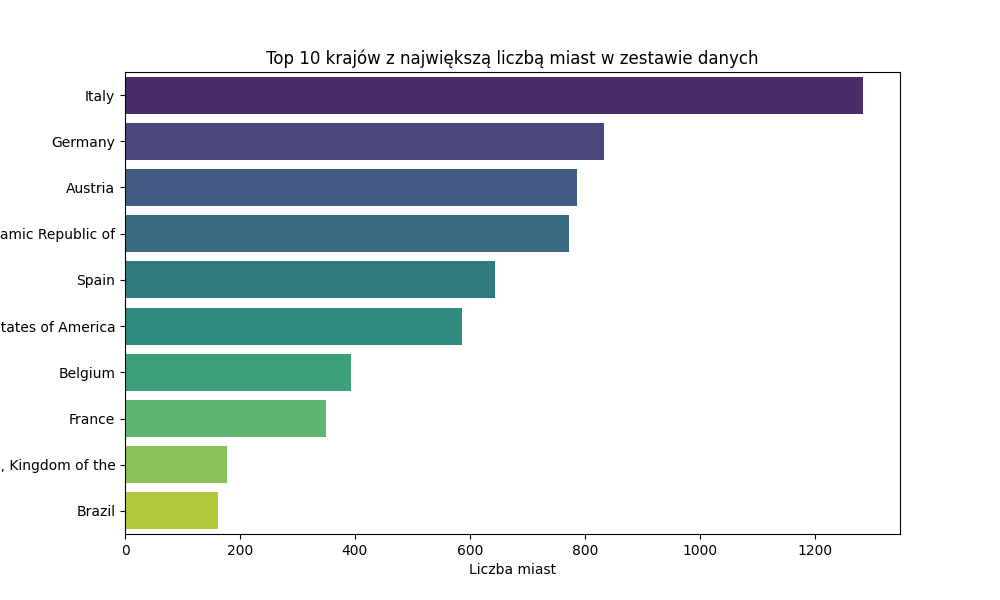
\includegraphics[scale=.3]{figs/top10countries.jpg}
    \caption{Top 10 krajów z największą liczbą miast w zestawie danych.}
    \label{FIG:top10countries}
\end{figure}

\begin{figure}[!htb]
    \centering
    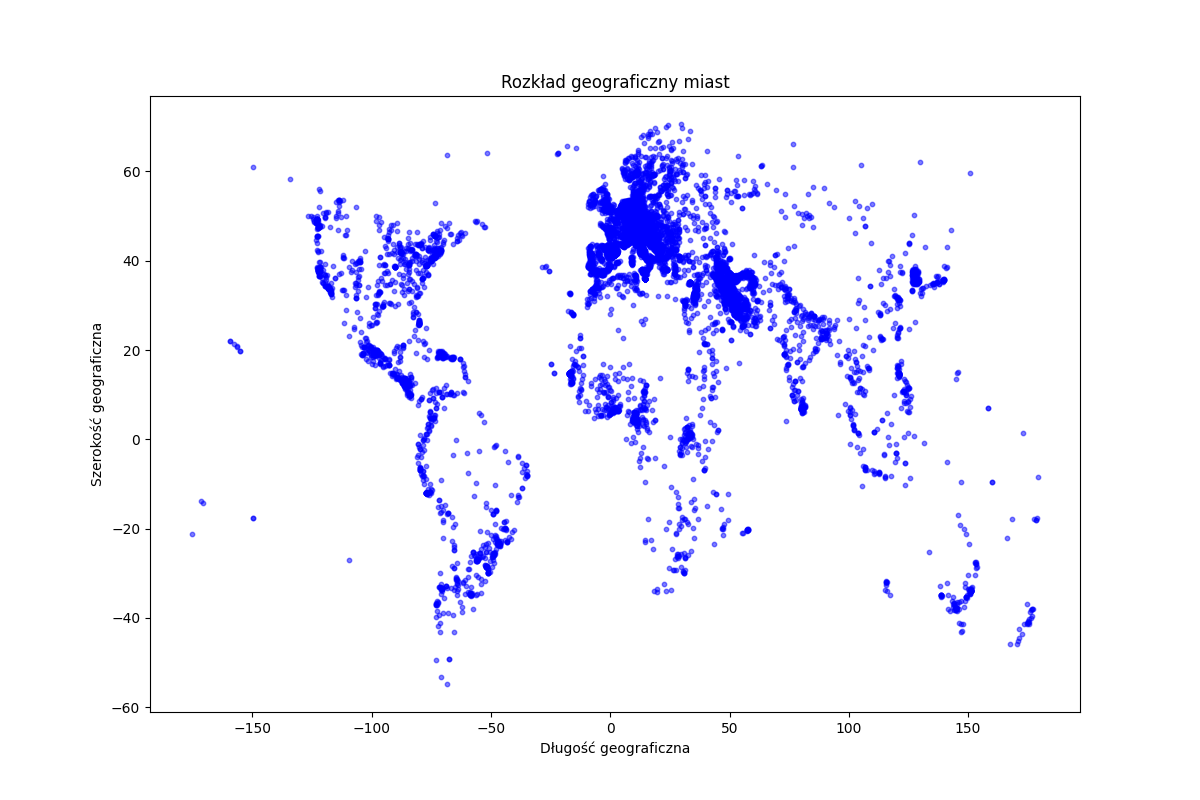
\includegraphics[scale=.3]{figs/Rozklad.png}
    \caption{Rozkład geograficzny miast członkowskich.}
    \label{FIG:geographical_distribution}
\end{figure}

\begin{figure}[!htb]
    \centering
    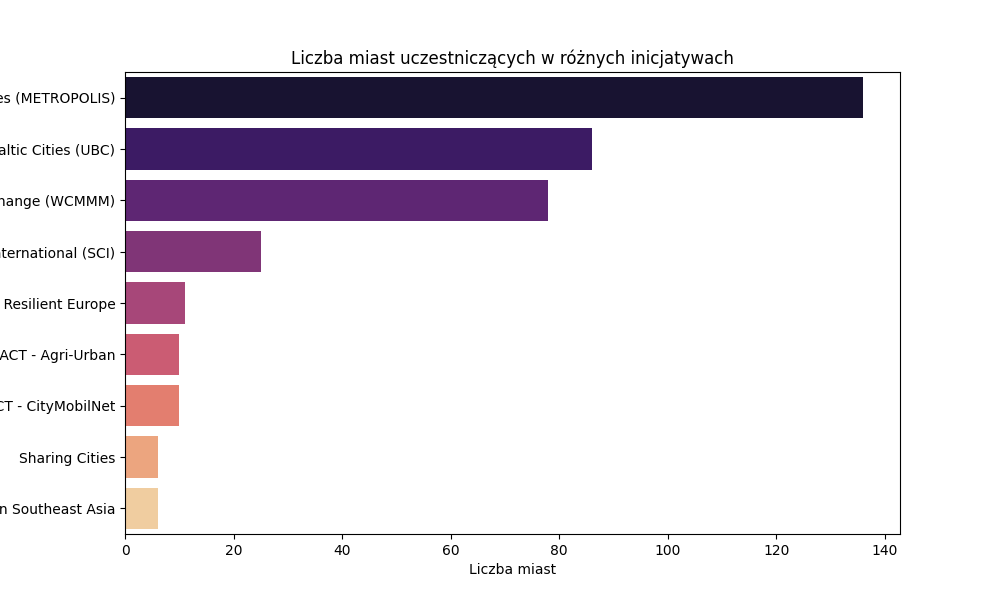
\includegraphics[scale=.3]{figs/Top10participants.png}
    \caption{Liczba miast uczestnicząca w różnych inicjatywach.}
    \label{FIG:initiatives_participation}
\end{figure}

\begin{figure}[!htb]
    \centering
    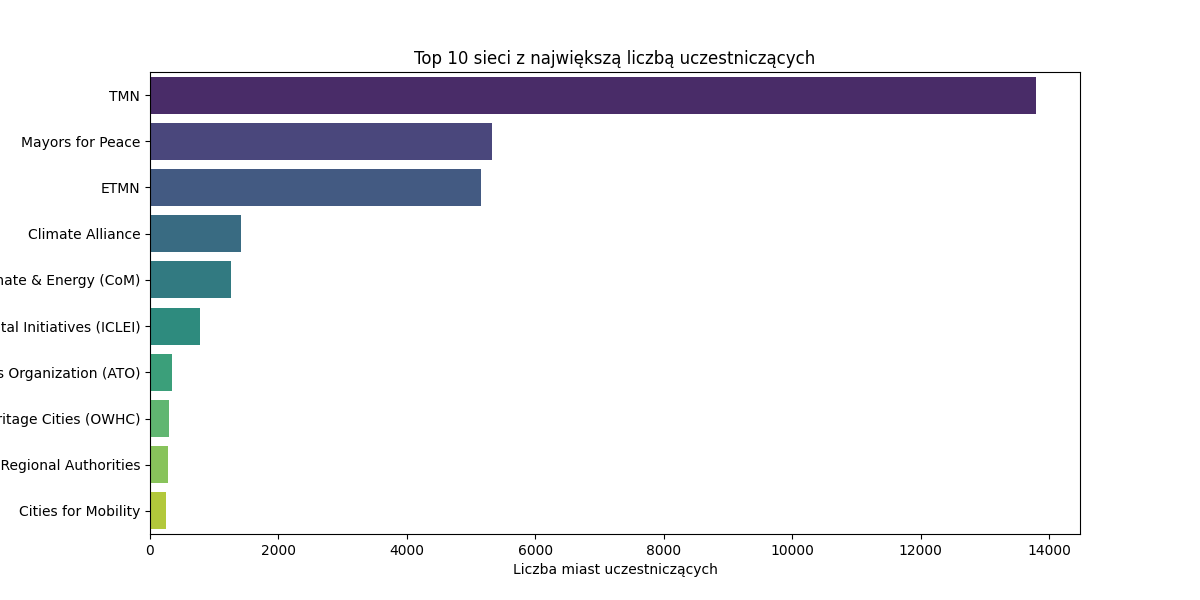
\includegraphics[scale=.3]{figs/Top10networks.png}
    \caption{Top 10 sieci z największą liczbą uczestniczących miast.}
    \label{FIG:top10networks}
\end{figure}




\section{Metodologia}
\subsection{Techniki analizy danych}
\textbf{K-means dla detekcji anomalii:} K-means jest algorytmem klasteryzacji, który grupuje dane w zbiory na podstawie ich podobieństwa. W tym przypadku zastosowano go do identyfikacji anomalii w zbiorze danych, gdzie mniejsze klastry mogą sugerować nietypowe zachowania. Proces obejmował następujące kroki:
---Wczytanie i normalizację danych (kolumny 'latitude.y', 'longitude.y', 'TMN', 'ETMN').
-Określenie optymalnej liczby klastrów za pomocą metody łokcia, a następnie trening modelu K-means z optymalną liczbą klastrów (w tym przypadku 5).
-Identyfikacja małych klastrów, które mogą wskazywać na anomalie, poprzez analizę rozmiarów klastrów.
-Wizualizacja rozmieszczenia geograficznego klastrów oraz anomalii, które zostały zidentyfikowane.


\begin{itemize}
\item[--] Wczytanie i normalizację danych (kolumny 'latitude.y', 'longitude.y', 'TMN', 'ETMN').
\item[--] Określenie optymalnej liczby klastrów za pomocą metody łokcia, a następnie trening modelu K-means z optymalną liczbą klastrów (w tym przypadku 5).
\item[--] Identyfikacja małych klastrów, które mogą wskazywać na anomalie, poprzez analizę rozmiarów klastrów.
\item[--] Wizualizacja rozmieszczenia geograficznego klastrów oraz anomalii, które zostały zidentyfikowane.
\end{itemize}


\textbf{Hierarchical Clustering:} Hierarchical Clustering to technika, która tworzy drzewo hierarchiczne (dendrogram) do analizy struktury danych. Dendrogram pozwala na wizualizację odległości między obiektami w zbiorze. W tym przypadku wykorzystano metodę Ward'a w połączeniu z analizą kategorii sub-regionów i sieci.
\begin{itemize}
\item[--] Znormalizowano dane numeryczne, a następnie stworzono dendrogram.
\item[--] Dokonano analizy zmienności sub-regionów i przypisano odpowiednie klastry do różnych obiektów.
\item[--] Wykorzystano PCA do wizualizacji klastrów w przestrzeni 2D oraz przeprowadzono detekcję anomalii przy użyciu Local Outlier Factor (LOF) i analizy odległości od centroidów.
\end{itemize}


\textbf{Clustering Sub-Regions and Networks:} Metoda ta polegała na podziale zbioru danych według subregionów geograficznych i specyficznych sieci TMNs. Zastosowanie algorytmu DBSCAN w celu analizy sub-regionów i sieci geograficznych:
\begin{itemize}
\item[--] Wykorzystano dane z kolumny sub-region, a także dane binarne związane z sieciami, które zostały znormalizowane.
\item[--] Dzięki PCA dokonano redukcji wymiarowości i wizualizacji klastrów.
\item[--] Dodatkowo, przeprowadzono detekcję anomalii w przestrzeni geograficznej (na podstawie długości i szerokości geograficznej), gdzie punkty oznaczone jako anomalie były reprezentowane na mapie.
\end{itemize}

\subsection{Uzasadnienie wyboru metod}
K-means: Został wybrany do wykrywania anomalii, ponieważ dobrze sprawdza się w identyfikacji nietypowych danych na podstawie liczby klastrów. Dzięki metodzie łokcia udało się określić optymalną liczbę klastrów, co jest kluczowe do dalszej analizy anomalii.

Hierarchical Clustering: Ta metoda pozwala na bardziej elastyczne grupowanie danych, bez konieczności wcześniejszego ustalania liczby klastrów. Jest szczególnie przydatna w analizie danych z bardziej złożoną strukturą hierarchiczną, jak sub-regiony. Użycie różnych metod linkowania (np. Ward, single, complete) pozwala na dostosowanie poziomu szczegółowości klasteryzacji.

DBSCAN: Wybrano ze względu na jego zdolność do wykrywania anomalii i klastra o nieregularnym kształcie. DBSCAN jest szczególnie skuteczny w przypadku, gdy dane są rozproszone i zawierają szumy, co sprawdza się w analizie sub-regionów oraz sieci. Algorytm pozwala na wyodrębnienie anomalii jako punkty, które nie należą do żadnego klastra.


\newpage
\section{Wyniki i dyskuja}
W ramach analizy wykrywania anomalii przy użyciu różnych metod klasteryzacji, takich jak K-means, Hierarchical Clustering oraz Sub-region/Network clustering, uzyskano różne wyniki, które pozwalają na wyciągnięcie istotnych wniosków.
\subsection{K-means}
Metoda K-means wykryła 147 anomalii. Wykorzystując algorytm K-means, podzieliliśmy dane na pięć klastrów, a anomalie zostały zidentyfikowane jako małe klastry o niskiej liczbie punktów. Obserwujemy, że ta metoda skutecznie grupuje dane, ale nie jest idealna w wykrywaniu bardzo małych anomalii, które mogą być istotne w kontekście specyficznych przypadków.
\begin{figure}[!htb]
    \centering
        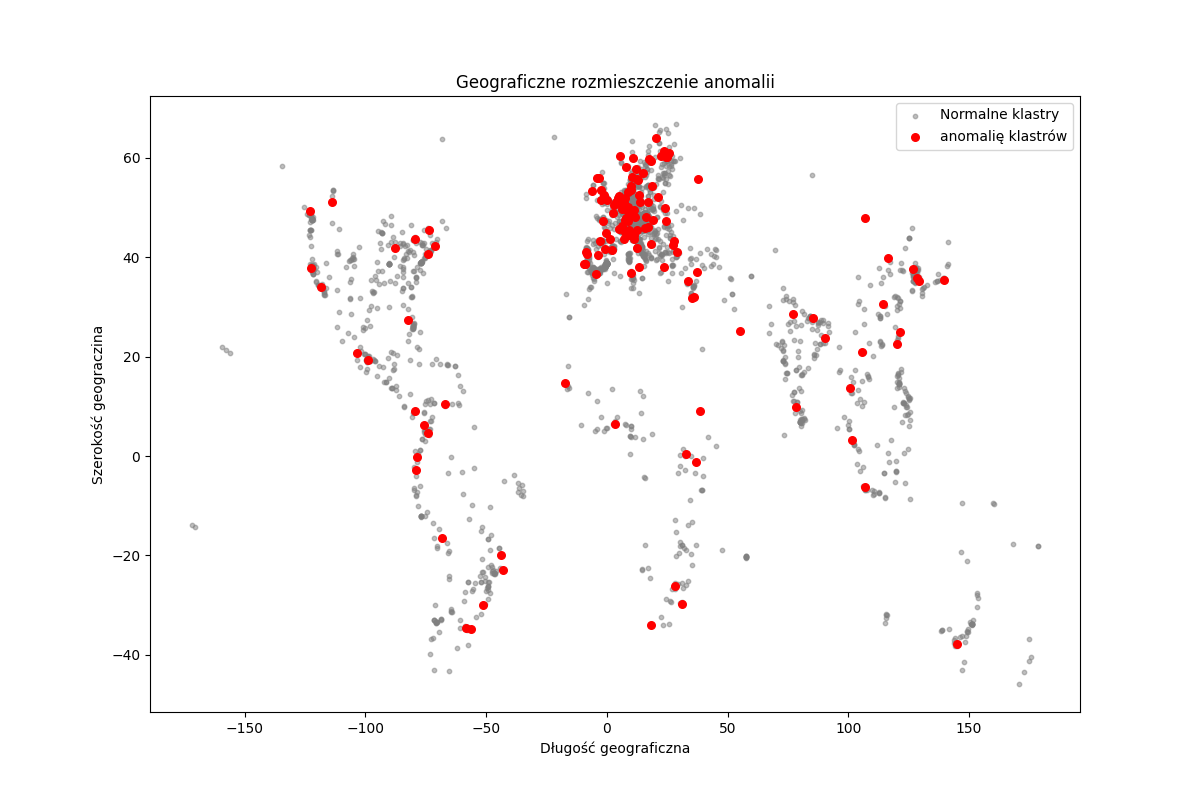
\includegraphics[scale=.3]{figs/AnomaliaKmeans.png}
    \caption{Graficzne rozmieszczenie anomalii K-means.}
    \label{FIG:AnomaliaKmeans}
\end{figure}
\subsection{Hierarchical Clustering}
Hierarchiczne grupowanie danych wykazało znacznie mniejszą liczbę anomalii – 5 anomalii. Zastosowanie tego algorytmu pozwala na lepsze zrozumienie struktury hierarchicznej danych i może być przydatne, gdy zależy nam na analizie relacji między obiektami na różnych poziomach. Mimo to, liczba wykrytych anomalii w tym przypadku była bardzo mała, co sugeruje, że metoda ta może być bardziej konserwatywna w identyfikowaniu nieprawidłowości.
\begin{figure}[!htb]
    \centering
        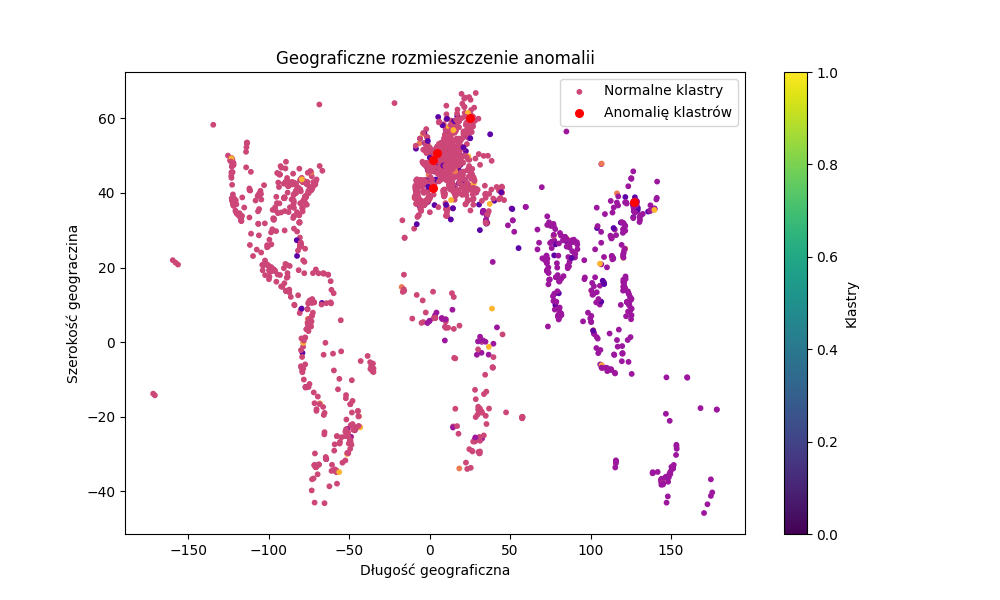
\includegraphics[width=0.5\textwidth, height=0.17\textheight]{figs/AnomaliaHierarchical.png}
    \caption{Graficzne rozmieszczenie anomalii Hierarchical Clustering.}
    \label{FIG:AnomaliaHierarchical}
\end{figure}
\FloatBarrier
\subsection{Sub-region/Network Clustering (DBSCAN)}
W przypadku analizy z wykorzystaniem algorytmu DBSCAN dla sub-regionów i sieci, wykryto aż 996 anomalii. DBSCAN jest bardziej elastyczny w wykrywaniu anomalii, szczególnie w danych, które mogą zawierać szumy lub nie mają wyraźnych granic między klastrami. Zidentyfikowanie tak dużej liczby anomalii może świadczyć o tym, że dane są bardziej rozproszone i zawierają więcej nietypowych punktów, które nie pasują do standardowych klastrów.
\begin{figure}[!htb]
    \centering
        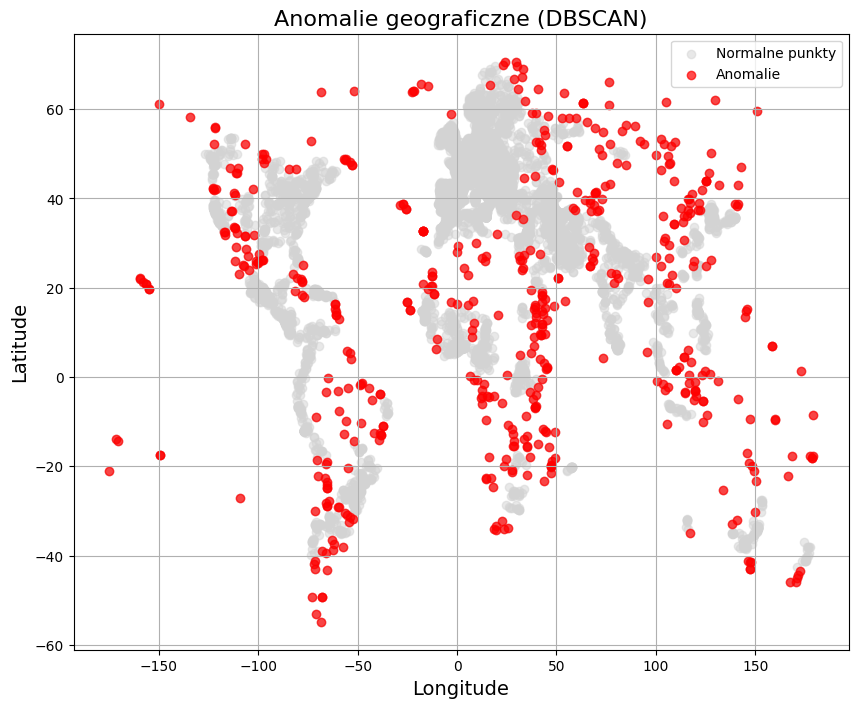
\includegraphics[scale=.3]{figs/AnomaliaSRNN.png}
    \caption{Graficzne rozmieszczenie anomalii Sub-region/Network Clustering.}
    \label{FIG:AnomaliaSRNN}
\end{figure}
\FloatBarrier
\section{Znaczenie wykrytych anomalii}
Wykrywanie anomalii w zbiorach danych jest kluczowym zadaniem w wielu dziedzinach, w tym w analizie danych przestrzennych, monitoringu sieci, oraz analizie systemów miejskich. Zidentyfikowane anomalie mogą dostarczyć cennych informacji na temat nietypowych, podejrzanych lub nieprawidłowych zdarzeń, które wymagają dalszej uwagi. Oto kilka aspektów, które podkreślają znaczenie wykrytych anomalii:
\subsection{Identyfikacja nieprawidłowości i potencjalnych zagrożeń}
Anomalie mogą wskazywać na występowanie nieprawidłowości w systemach, które mogą prowadzić do poważnych problemów, takich jak awarie, błędy w danych, czy incydenty bezpieczeństwa. Na przykład, w analizie sieci miejskich, anomalie w danych geograficznych mogą wskazywać na nieautoryzowane lub nieprawidłowe działania, które mogą stanowić zagrożenie dla integralności systemu.
\subsection{Optymalizacja zarządzania i podejmowanie decyzji}
Wykrywanie anomalii może pomóc w optymalizacji zarządzania zasobami. Na przykład, w systemach miejskich, anomalie w danych o ruchu drogowym mogą wskazywać na nieefektywności w infrastrukturze transportowej, umożliwiając wprowadzenie poprawek w celu poprawy płynności ruchu i redukcji korków. Dzięki temu władze lokalne mogą podejmować lepsze decyzje w zakresie rozwoju infrastruktury.
\subsection{Wykrywanie oszustw i nadużyć}
W kontekście analizy sieci społecznych lub transakcji, anomalie mogą wskazywać na podejrzane zachowania lub oszustwa. Na przykład, w systemach bankowych, wykrycie nieprawidłowych wzorców w transakcjach może pomóc w identyfikacji oszustw finansowych. Analiza anomalii pozwala na wczesne wykrycie i zapobieganie niepożądanym zdarzeniom.
\subsection{Doskonalenie algorytmów i modeli analitycznych}
Wykryte anomalie mogą również służyć jako przypadki testowe do udoskonalania algorytmów wykrywania anomalii. Przez analizę anomalii w różnych metodach klasteryzacji (takich jak K-means, DBSCAN czy Hierarchical Clustering), możemy lepiej zrozumieć, które podejście jest najbardziej efektywne w danym kontekście, a także które rodzaje anomalii są najbardziej istotne do dalszej analizy.


\section{Wnioski}
W przeprowadzonej analizie wykrywania anomalii przy użyciu różnych metod klasteryzacji, takich jak K-means, Hierarchical Clustering oraz Sub-region Clustering, uzyskano interesujące wyniki, które mogą przyczynić się do lepszego zrozumienia struktury i nieprawidłowości w badanym zbiorze danych. Oto kluczowe wnioski:
\subsection{Porównanie liczby anomalii}
K-means: Metoda K-means wykryła 147 anomalii, co wskazuje na obecność licznych, nietypowych punktów w zbiorze danych. Choć K-means jest skuteczny w segmentowaniu danych, wyniki te mogą być efektem zbyt dużej liczby klastrów, w których dane są podzielone na zbyt małe grupy.

Hierarchical Clustering: Ta metoda wykryła tylko 5 anomalii, co sugeruje, że struktura danych jest bardziej spójna i hierarchiczna. Hierarchical Clustering, dzięki swojej zdolności do analizowania danych na różnych poziomach, może lepiej identyfikować naturalne grupy w danych i w tym przypadku wykryć mniej, ale bardziej istotnych anomalii.

Sub-region Clustering: Wykryto 996 anomalii, co wskazuje na bardzo zróżnicowaną strukturę w obrębie różnych podregionów. Taki wynik może sugerować, że dane w obrębie podregionów są mocno zróżnicowane, a zmienność w tych obszarach jest większa niż w innych metodach klasteryzacji.
\subsection{Wizualizacja anomalii}
Wizualizacje wykazały, że w każdym przypadku anomalie są rozmieszczone w różnych częściach danych. W przypadku K-means i Sub-region Clustering, anomalie były bardziej rozproszone w przestrzeni, co może świadczyć o bardziej rozdrobnionych strukturach w tych metodach. Z kolei w Hierarchical Clustering anomalie były bardziej skonsolidowane, co odzwierciedla spójną strukturę w danych.
\subsection{Różnice w efektywności metod}
K-means, mimo dużej liczby anomalii, może nie być najefektywniejszą metodą do wykrywania nieprawidłowości w tego typu danych, ze względu na swoją tendencję do dzielenia danych na zbyt małe grupy. W przeciwieństwie do tego, Hierarchical Clustering wykazał się większą precyzją, wykrywając jedynie kluczowe anomalie, które były bardziej reprezentatywne dla rozkładu danych.
Sub-region Clustering, z uwagi na analizę danych w kontekście podregionów, okazał się najbardziej podatny na wykrywanie większej liczby anomalii, co może wynikać z dużej zmienności w obrębie poszczególnych regionów.
\subsection{Znaczenie wyników w kontekście dalszej analizy}
Wykryte anomalie w różnych metodach mogą stanowić punkt wyjścia do dalszej analizy, w tym identyfikacji przyczyn tych nieprawidłowości oraz potencjalnych działań naprawczych. W zależności od kontekstu, można uznać, że metoda Hierarchical Clustering dostarcza najbardziej wartościowych wyników, gdyż identyfikuje mniej, ale bardziej krytyczne anomalie, które mogą mieć większe znaczenie dla struktury badanych danych.
Dalsze badania mogą obejmować testowanie innych metod wykrywania anomalii oraz zastosowanie bardziej zaawansowanych technik, takich jak analiza outlierów w kontekście różnych zmiennych, aby lepiej zrozumieć, dlaczego te anomalie występują.
\subsection{Zastosowanie wyników w praktyce}
Wyniki wykrywania anomalii mają potencjał do zastosowań w różnych dziedzinach, takich jak monitoring sieci miejskich, analiza bezpieczeństwa, a także w obszarze optymalizacji zarządzania zasobami. Zidentyfikowanie nieprawidłowości może pomóc w podejmowaniu szybszych decyzji operacyjnych oraz w opracowywaniu strategii naprawczych.
%% Loading bibliography style file
%\bibliographystyle{model1-num-names}
\newpage
\bibliographystyle{cas-model2-names}

% Loading bibliography database
\bibliography{bibliografia}

\end{document}

